\documentclass{amsart}
%DIF LATEXDIFF DIFFERENCE FILE
%DIF DEL report01.tex    Fri Jan 15 19:39:36 2021
%DIF ADD report01q.tex   Fri Jan 15 21:12:04 2021
\synctex=1

%=================================================================
% 
\newcount\DraftStatus  % 0 suppresses notes to selves in text
\DraftStatus=1   % TODO: set to 0 for final version
%=================================================================

%=================================================================
\usepackage{comment}
%=================================================================
%
\includecomment{JournalOnly}  
\includecomment{ConferenceOnly}  
\includecomment{TulipStyle}
%
%=================================================================
\input{preamble}


%=================================================================
%
%DIF PREAMBLE EXTENSION ADDED BY LATEXDIFF
%DIF UNDERLINE PREAMBLE %DIF PREAMBLE
\RequirePackage[normalem]{ulem} %DIF PREAMBLE
\RequirePackage{color}\definecolor{RED}{rgb}{1,0,0}\definecolor{BLUE}{rgb}{0,0,1} %DIF PREAMBLE
\providecommand{\DIFadd}[1]{{\protect\color{blue}\uwave{#1}}} %DIF PREAMBLE
\providecommand{\DIFdel}[1]{{\protect\color{red}\sout{#1}}}                      %DIF PREAMBLE
%DIF SAFE PREAMBLE %DIF PREAMBLE
\providecommand{\DIFaddbegin}{} %DIF PREAMBLE
\providecommand{\DIFaddend}{} %DIF PREAMBLE
\providecommand{\DIFdelbegin}{} %DIF PREAMBLE
\providecommand{\DIFdelend}{} %DIF PREAMBLE
\providecommand{\DIFmodbegin}{} %DIF PREAMBLE
\providecommand{\DIFmodend}{} %DIF PREAMBLE
%DIF FLOATSAFE PREAMBLE %DIF PREAMBLE
\providecommand{\DIFaddFL}[1]{\DIFadd{#1}} %DIF PREAMBLE
\providecommand{\DIFdelFL}[1]{\DIFdel{#1}} %DIF PREAMBLE
\providecommand{\DIFaddbeginFL}{} %DIF PREAMBLE
\providecommand{\DIFaddendFL}{} %DIF PREAMBLE
\providecommand{\DIFdelbeginFL}{} %DIF PREAMBLE
\providecommand{\DIFdelendFL}{} %DIF PREAMBLE
%DIF LISTINGS PREAMBLE %DIF PREAMBLE
\RequirePackage{listings} %DIF PREAMBLE
\RequirePackage{color} %DIF PREAMBLE
\lstdefinelanguage{DIFcode}{ %DIF PREAMBLE
%DIF DIFCODE_UNDERLINE %DIF PREAMBLE
  moredelim=[il][\color{red}\sout]{\%DIF\ <\ }, %DIF PREAMBLE
  moredelim=[il][\color{blue}\uwave]{\%DIF\ >\ } %DIF PREAMBLE
} %DIF PREAMBLE
\lstdefinestyle{DIFverbatimstyle}{ %DIF PREAMBLE
	language=DIFcode, %DIF PREAMBLE
	basicstyle=\ttfamily, %DIF PREAMBLE
	columns=fullflexible, %DIF PREAMBLE
	keepspaces=true %DIF PREAMBLE
} %DIF PREAMBLE
\lstnewenvironment{DIFverbatim}{\lstset{style=DIFverbatimstyle}}{} %DIF PREAMBLE
\lstnewenvironment{DIFverbatim*}{\lstset{style=DIFverbatimstyle,showspaces=true}}{} %DIF PREAMBLE
%DIF END PREAMBLE EXTENSION ADDED BY LATEXDIFF

\begin{document}
%
%=================================================================
%
\title[A Short Running Title]{ What's Cooking}%

\author{Jincai Ma}



%\thanks{Thanks to \ldots}%
\subjclass{What's Cooking}%
\keywords{Application software learning, Kaggle topic selection}%
\date{\gitAuthorDate}%

\begin{abstract}
    The project\DIFaddbegin \DIFadd{(What's Cooking) }\DIFaddend will use the data set provided by Yummly to train and test a model and test its performance and predictive power.A good model trained by this data can be used  \DIFdelbegin \DIFdel{to predict the }\DIFdelend cuisine.The dataset for this project is from the Kaggle What's Cooking competition.A total of 39,774/9,944 training and test data points, covering information on Chinese, Vietnamese, French, etc.

\end{abstract}

\maketitle
\tableofcontents

\newpage
%=================================================================

%=================================================================
\section{Introduction}
\label{sec-intro}
   (1)Use recipe ingredients to categorize the cuisine.
   Given the name of the condiment, predict the cuisine to which the dish belongs.\\
   (2)The data comes from Kaggle https://www.kaggle.com/c/bike-sharing-demand.\\
   (3) In the dataset,including the recipe ID, the dish, and the list of ingredients for each recipe (variable length).The data is stored in JSON format. \\
   1.train.json- A training set that contains the recipe ID, dish type, and ingredient list
   2.test.json- A test set containing a recipe ID and a list of ingredients
   3.sample_submission.csv-Properly formatted sample submission document
\section{Data Analysis} \label{sec-preliminaries}

First of all, our work can be divided into the following steps:\\
(1)   Data Import And Introduction:\\a.Import the JSON file with Pandas:
We can get the data set of dish names, including 39774 training data and 9944 test samples.To see the distribution of our data set and the total variety of dishes, we printed out some of the data samples.
\begin{center}
  \begin{minipage}{1\linewidth}
  \centering
  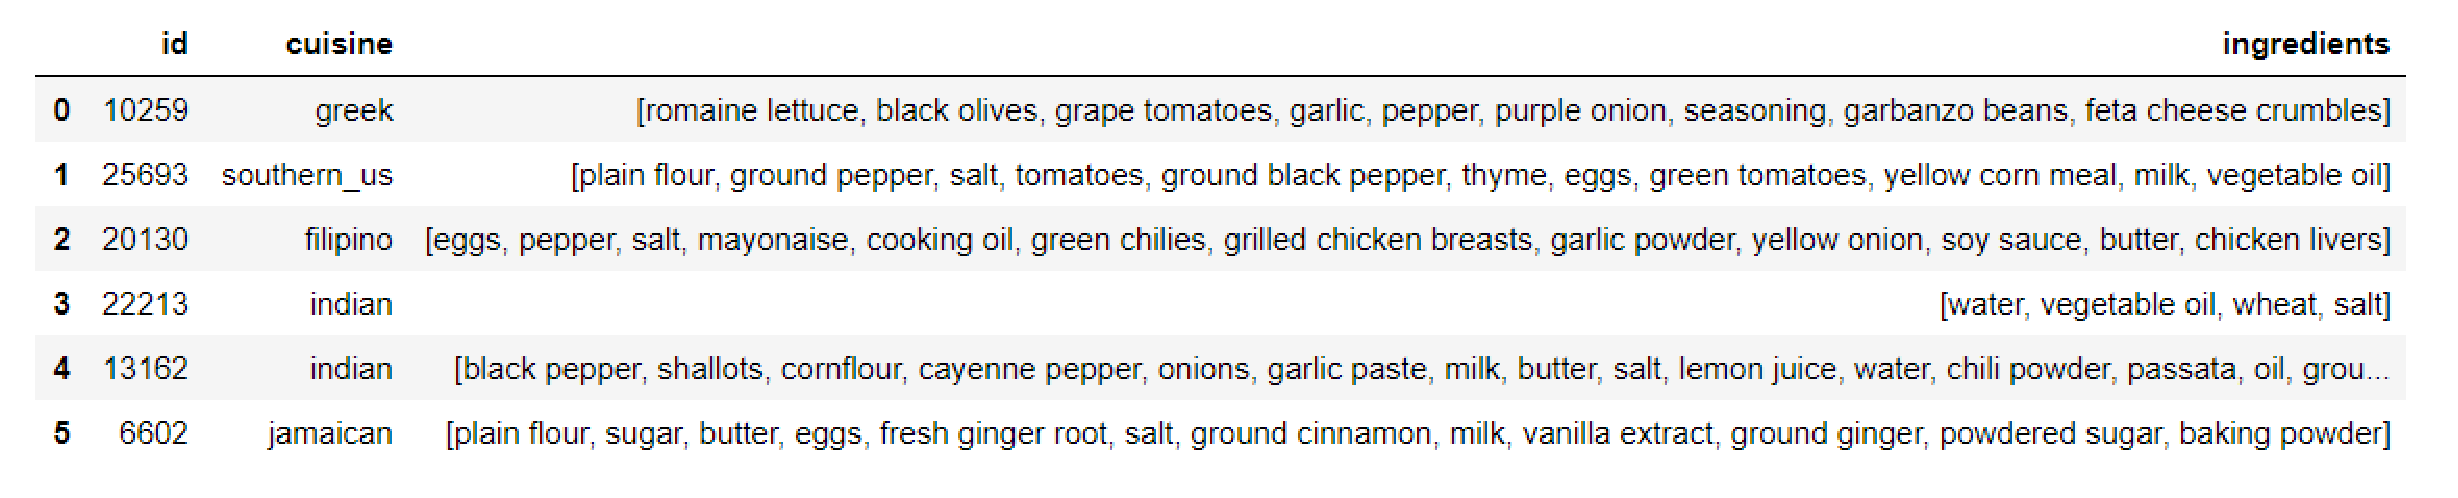
\includegraphics[width=0.6\textwidth]{pic01/a .eps}
  \end{minipage}
  b.Total dish classification\\
        There are 20 dishes in total, which are:
        ['brazilian' 'british' 'cajun_creole' 'chinese' 'filipino' 'french'
         'greek' 'indian' 'irish' 'italian' 'jamaican' 'japanese' 'korean'
         'mexican' 'moroccan' 'russian' 'southern_us' 'spanish' 'thai'
         'vietnamese']
  \hfill
\end{center}

(2) a.The data set is divided into Features and Target Variables.\\
 b.Features:'ingredients', we were given the names of the ingredients contained in each dish;
Target variable:'cuisine', is the classification of cuisines that we want to predict.\\
c.Extract the Feature of training data set into train_integredients variable
      Extract the Target Variables into the train_Targets variable.
\begin{center}
  \begin{minipage}{1\linewidth}
  \centering
  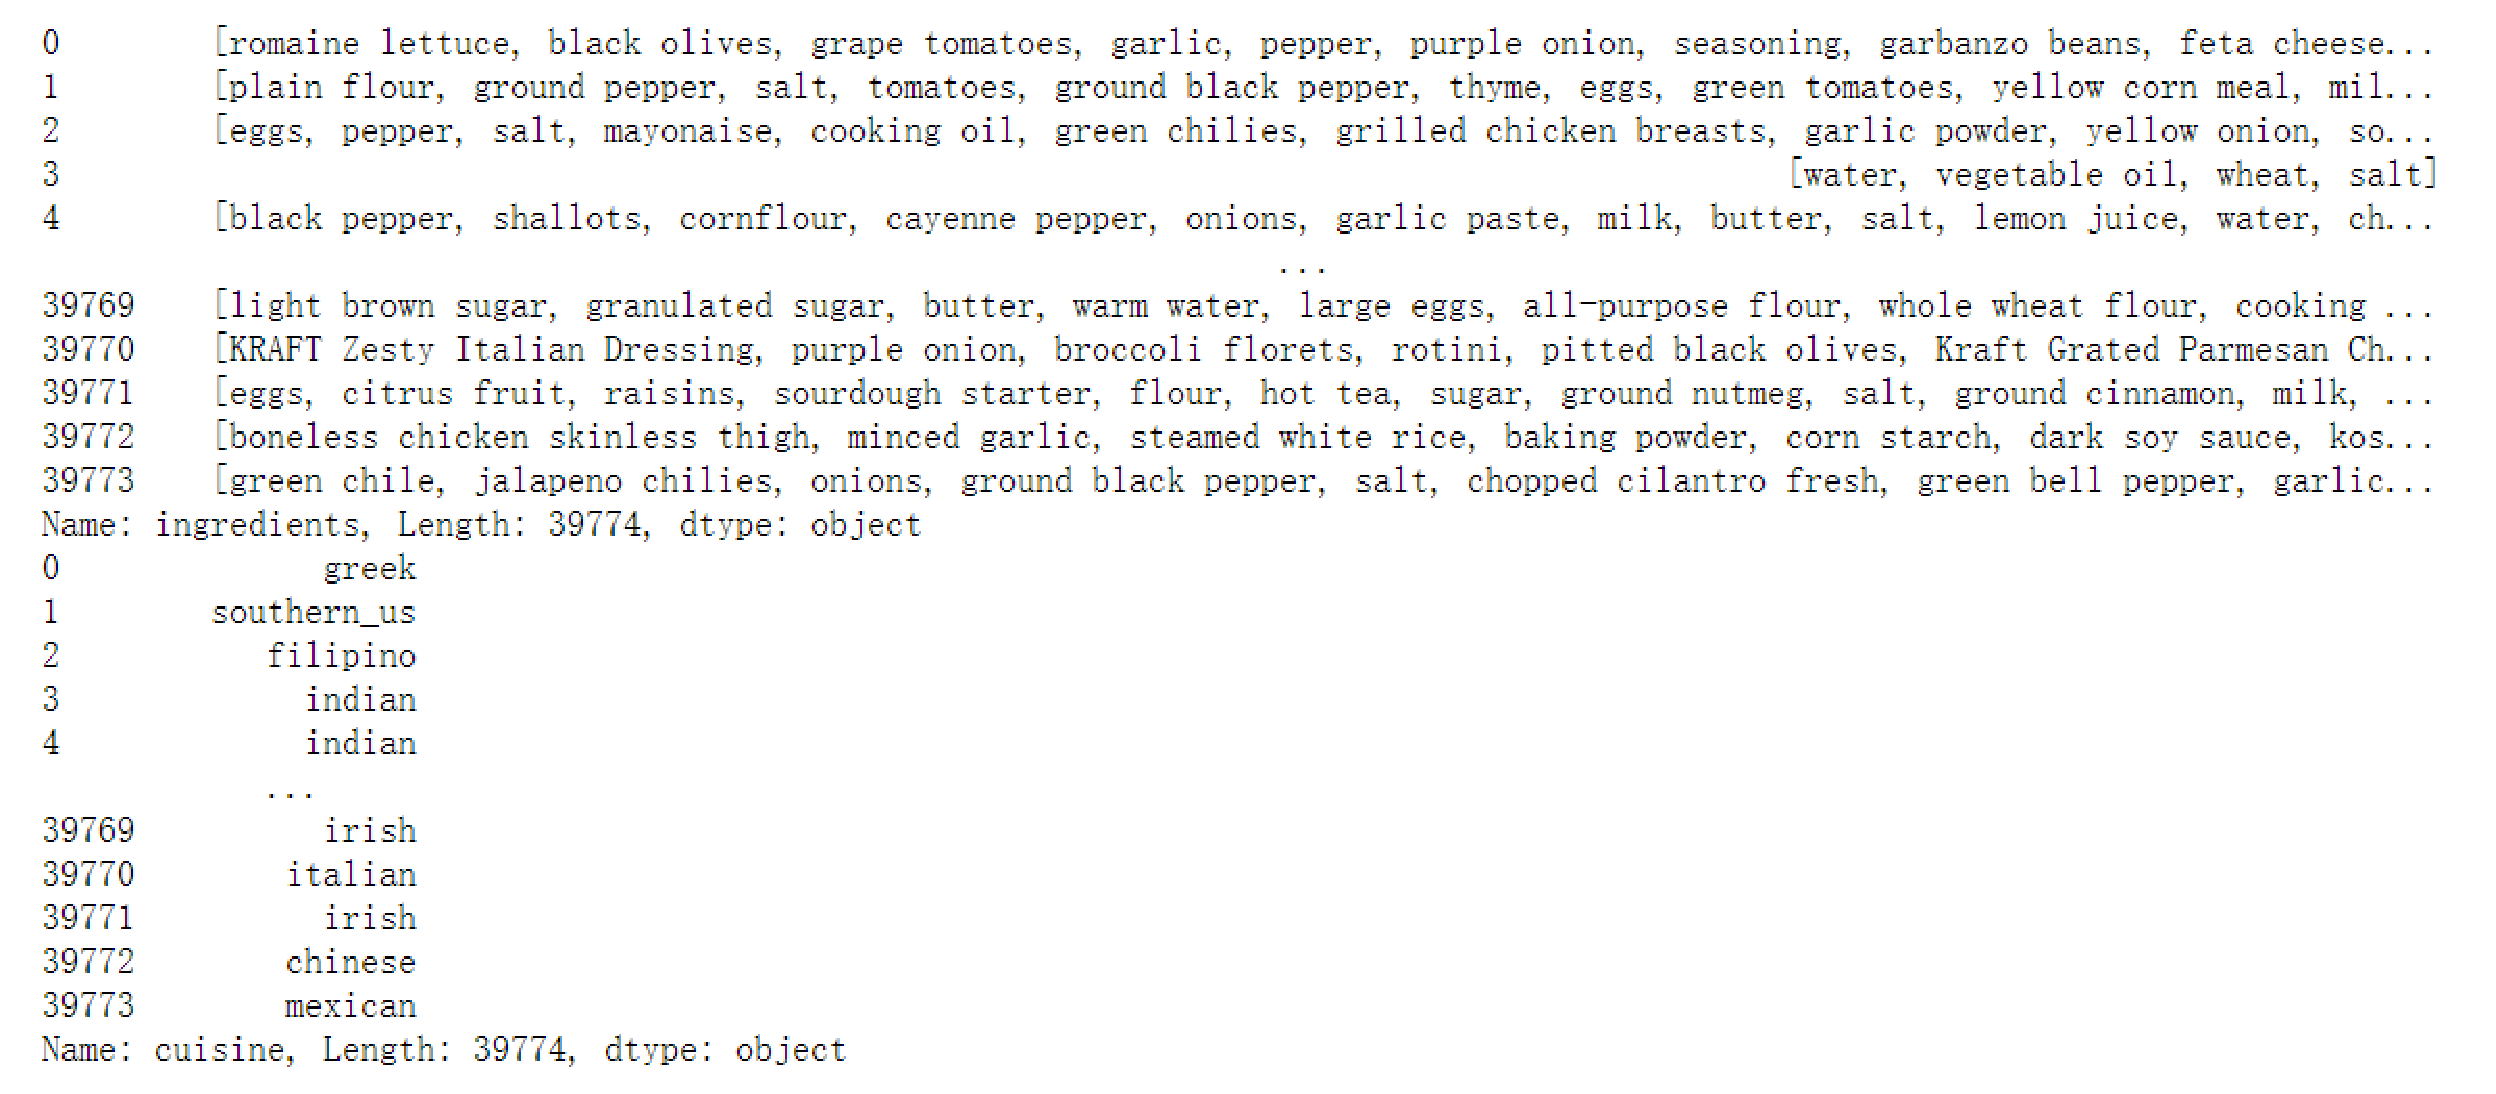
\includegraphics[width=0.7\textwidth]{pic01/b.eps}
\end{minipage}

  \hfill
\end{center}
(3) Data  Visualization:What are the top 10 most frequently used ingredients?\\ What are the 10 most common ingredients in filipino,greek and Italian cuisine?
\begin{center}
  \begin{minipage}{0.5\linewidth}
    \centering
    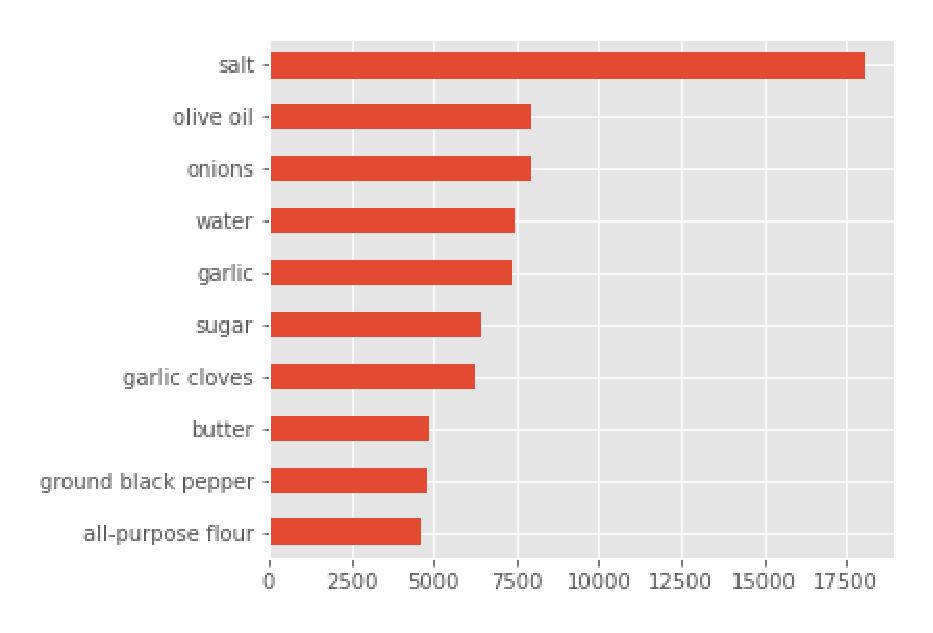
\includegraphics[width=0.5\textwidth]{pic01/cooking.eps}
  \end{minipage}
  
  \begin{minipage}{0.5\linewidth}
    \centering
    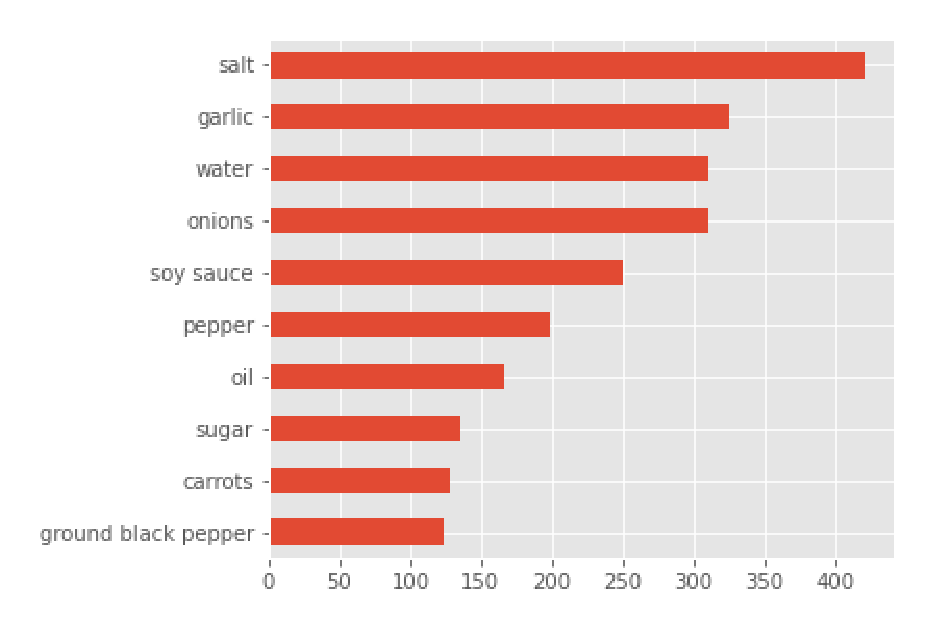
\includegraphics[width=0.5\textwidth]{pic01/filipino.eps}
  \end{minipage}
  
  \begin{minipage}{0.5\linewidth}
    \centering
      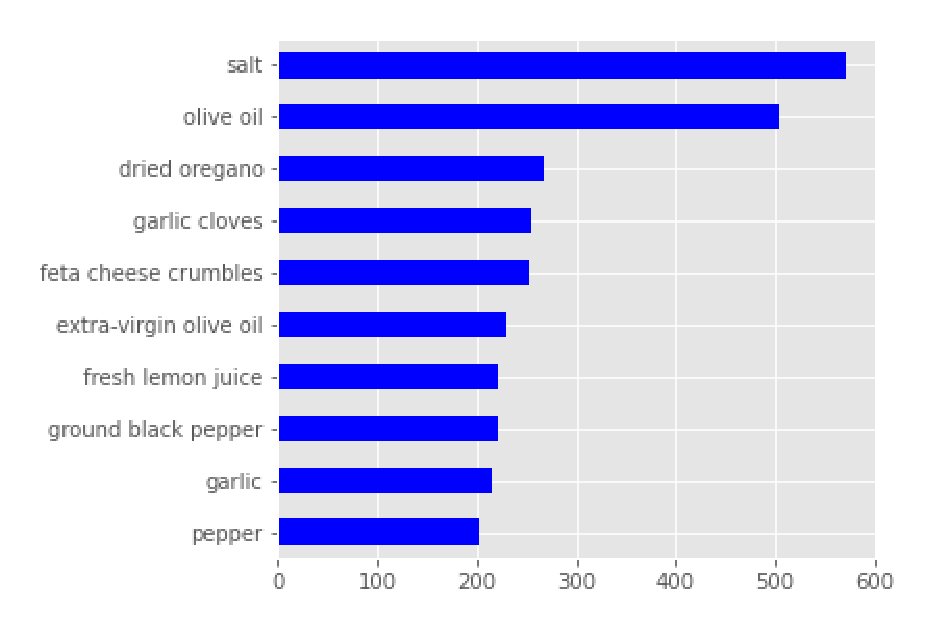
\includegraphics[width=0.5\textwidth]{pic01/greek.eps}
  \end{minipage}
  \begin{minipage}{0.5\linewidth}
    \centering
      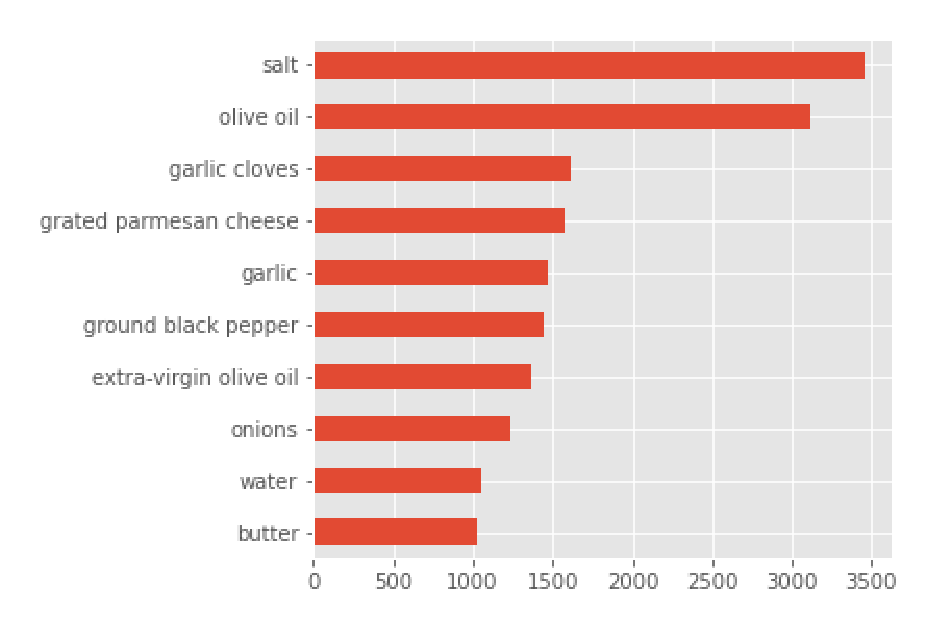
\includegraphics[width=0.5\textwidth]{pic01/italian.eps}
  \end{minipage}
  \hfill
\end{center}

(4)  Data Cleaning:Since dishes contain a large number of ingredients, and since the same ingredients can vary in numbers, tenses, and so on, we considered sifting through a potatos to remove any such differences.
\begin{center}
  \begin{minipage}{1\linewidth}
    \centering
    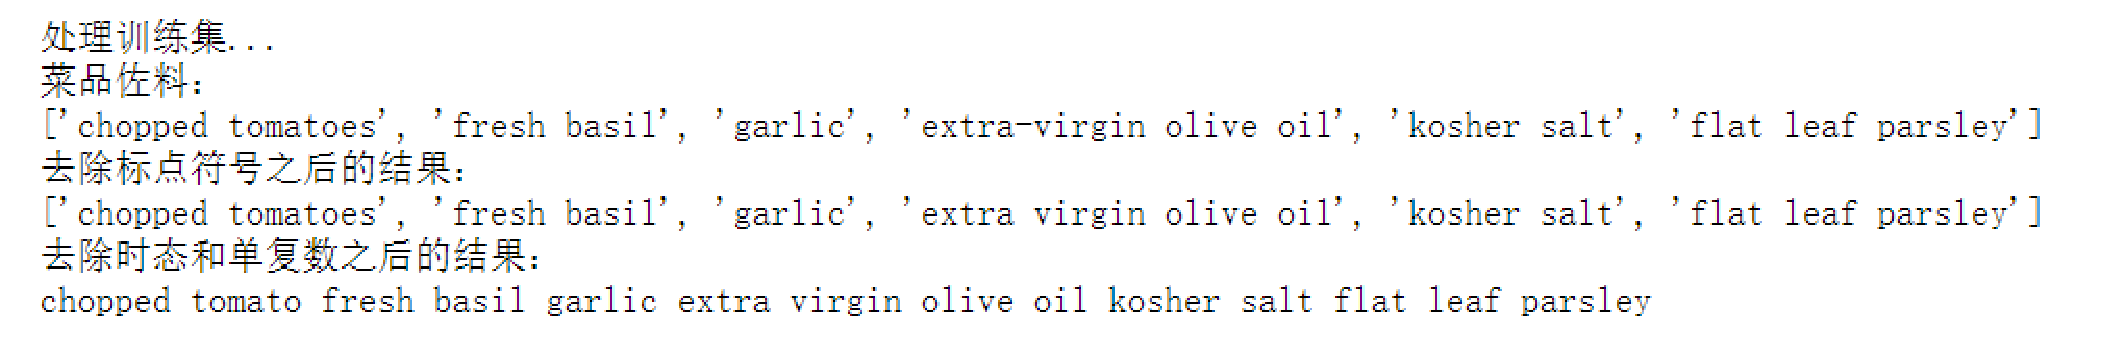
\includegraphics[width=0.9\textwidth]{pic01/clean1.eps}
  \end{minipage}
  \begin{minipage}{1\linewidth}
    \centering
    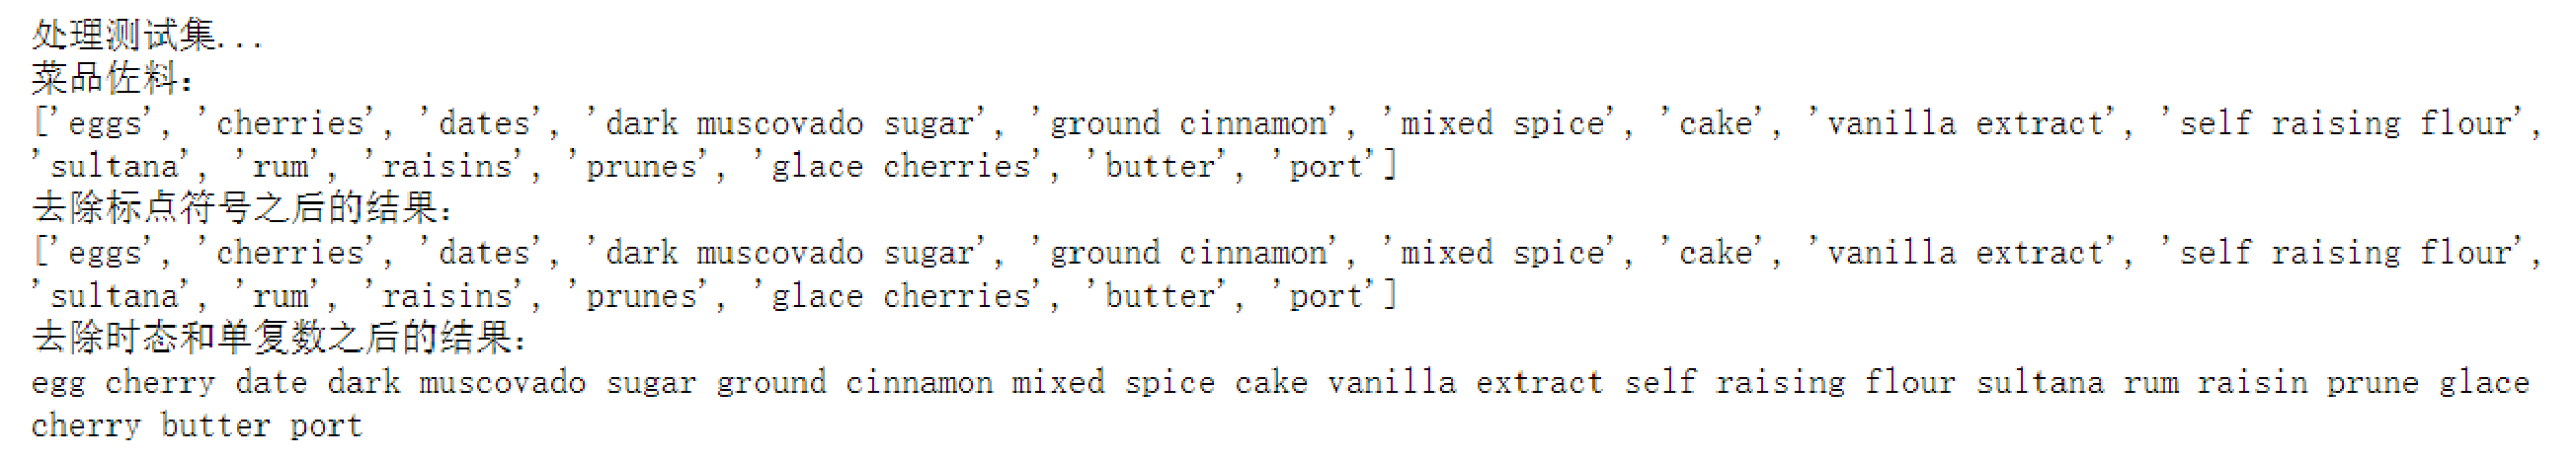
\includegraphics[width=0.9\textwidth]{pic01/clean2.eps}
  \end{minipage}
  
  \hfill
\end{center}




(5) Feature extraction:\\
a.We convert the ingredients of the dish into a numerical feature vector.Consider that most dishes include salt, water, sugar, butter, etc,We will consider weighting the seasonings according to the occurrence times of the seasonings, that is, the more the occurrence times of the condiments, the lower the discriminability of the condiments.The feature we adopt is TF-IDF.\\
b.We can get the characteristics:\lbrack'greek','southern\_us','filipino','indian','indian',\\
'jamaican','spanish','italian','mexican','italian'\rbrack
\begin{center}
  
  \hfill
\end{center}

(6)  The impact of weather

\begin{center}
  \begin{minipage}{0.7\linewidth}
    \centering
    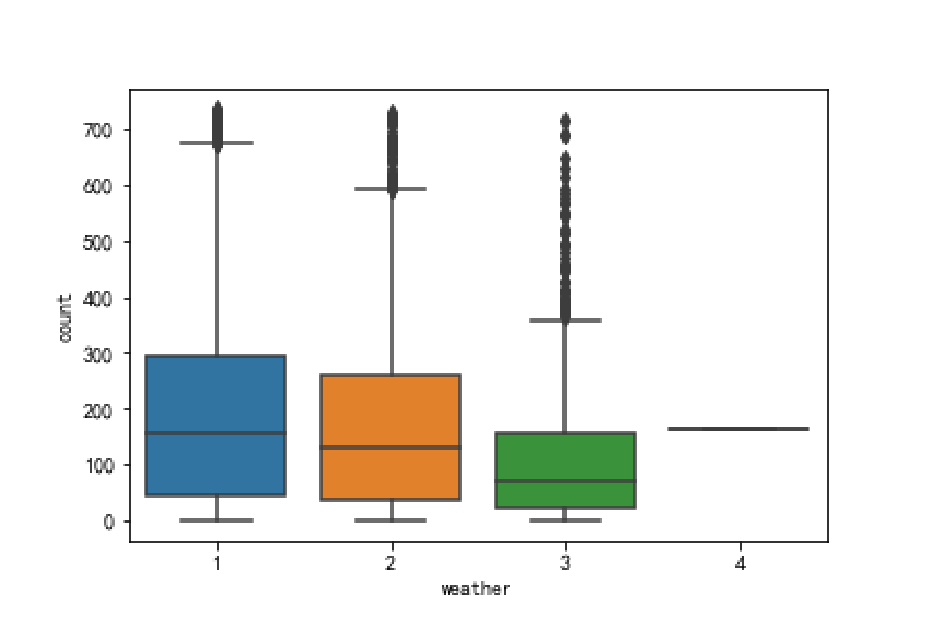
\includegraphics[height=0.7\textwidth]{pic/weather.eps}
  \end{minipage}
  \hfill
\end{center}

(7) Impact of season,week,registered and non-registered users on cycling usage trends\\
    a.For different times of the day, there is a clear trend in the use of Shared bikes, with two distinct peaks, in line with people's understanding of morning peak and evening peak.The trends were the same for all four seasons, except that usage in spring was slightly lower than in the other three.
\begin{center}
  \begin{minipage}{1\linewidth}
    \centering
    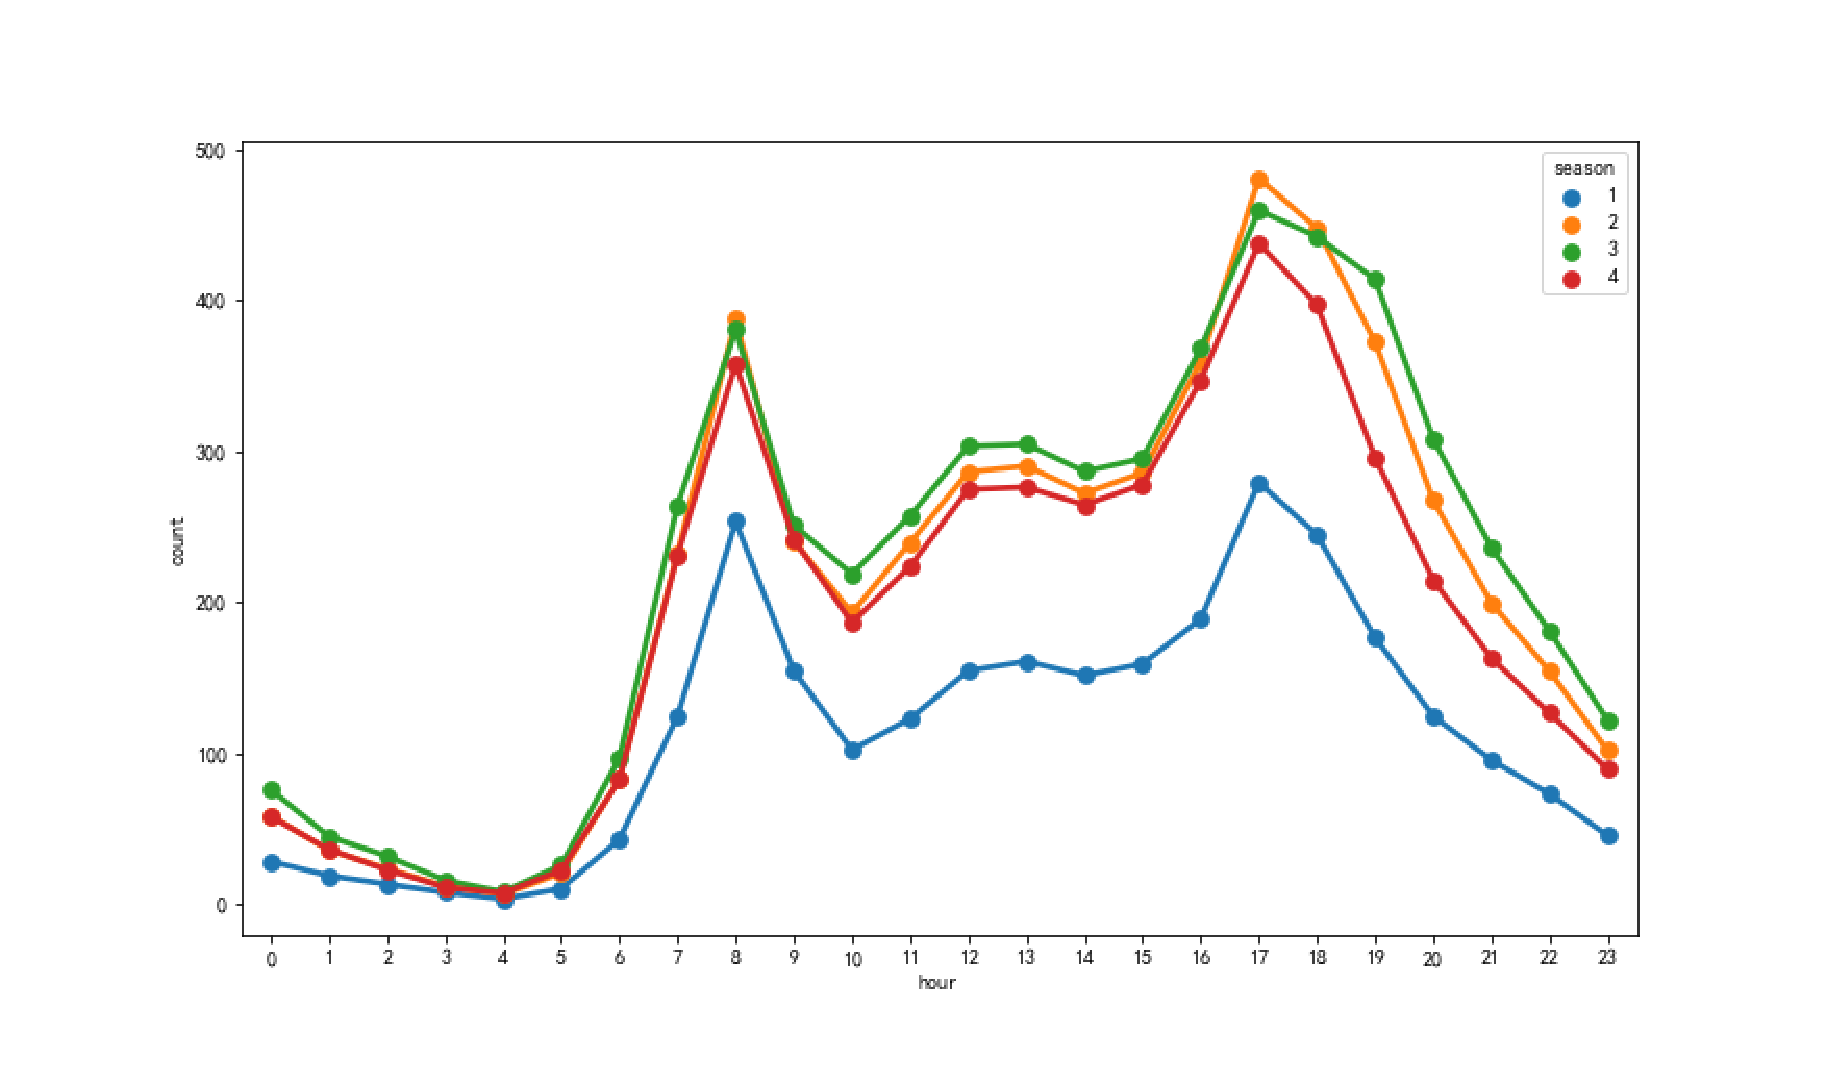
\includegraphics[width=0.7\textwidth]{pic/three hour1 (2).eps}
  \end{minipage}
  
  
  \hfill
\end{center}
b.The usage of registered users accounts for the majority of the total usage, and the trend is consistent with the total usage trend, rather than that of registered users. The usage at different times of the day does not change much, and the trend is similar to the usage trend at weekends.
\begin{center}
  \begin{minipage}{1\linewidth}
    \centering
    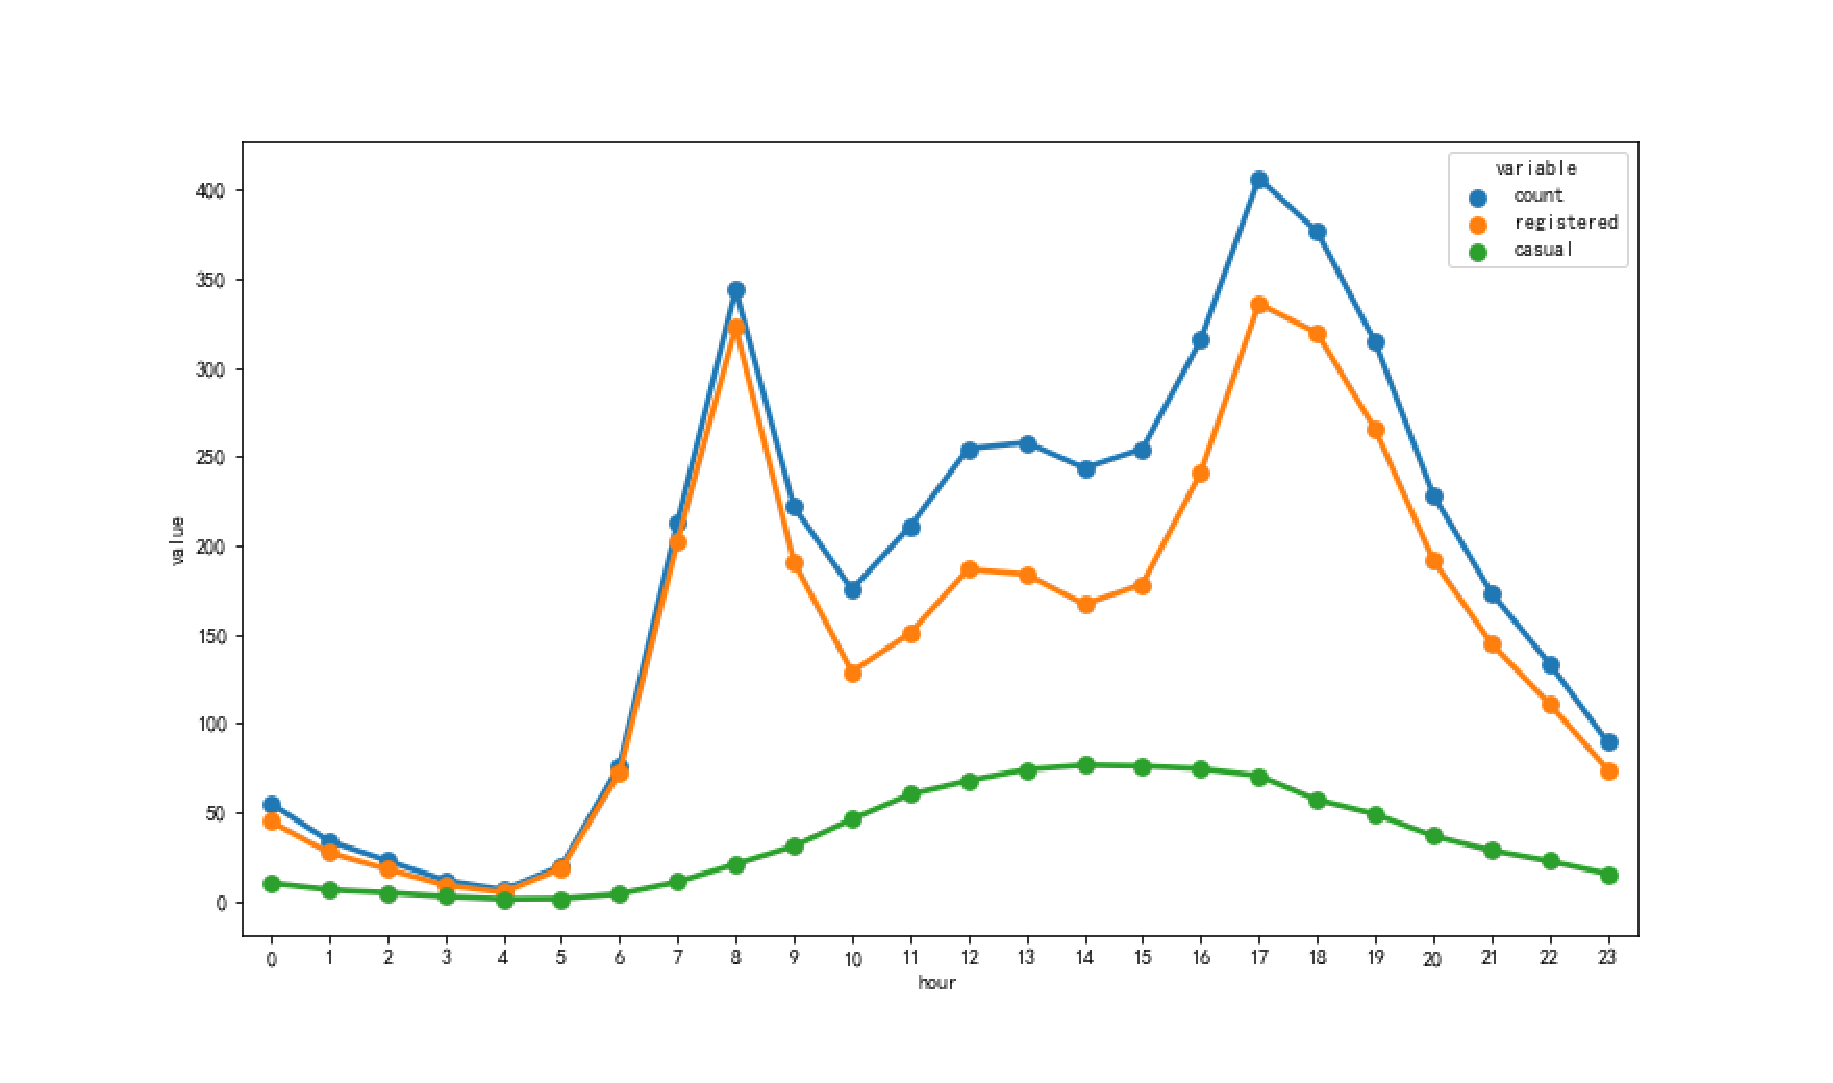
\includegraphics[width=0.7\textwidth]{pic/three hour3.eps}
  \end{minipage}
  \hfill
\end{center}
 
c.From Monday to Friday, there are two peak usage periods, while on weekends, the usage trend is completely different from that on weekdays. The usage trend changes from bimodal to flat unimodal, and the peak usage period is concentrated at 11-17 o 'clock.
\begin{center}
  \begin{minipage}{1\linewidth}
    \centering
    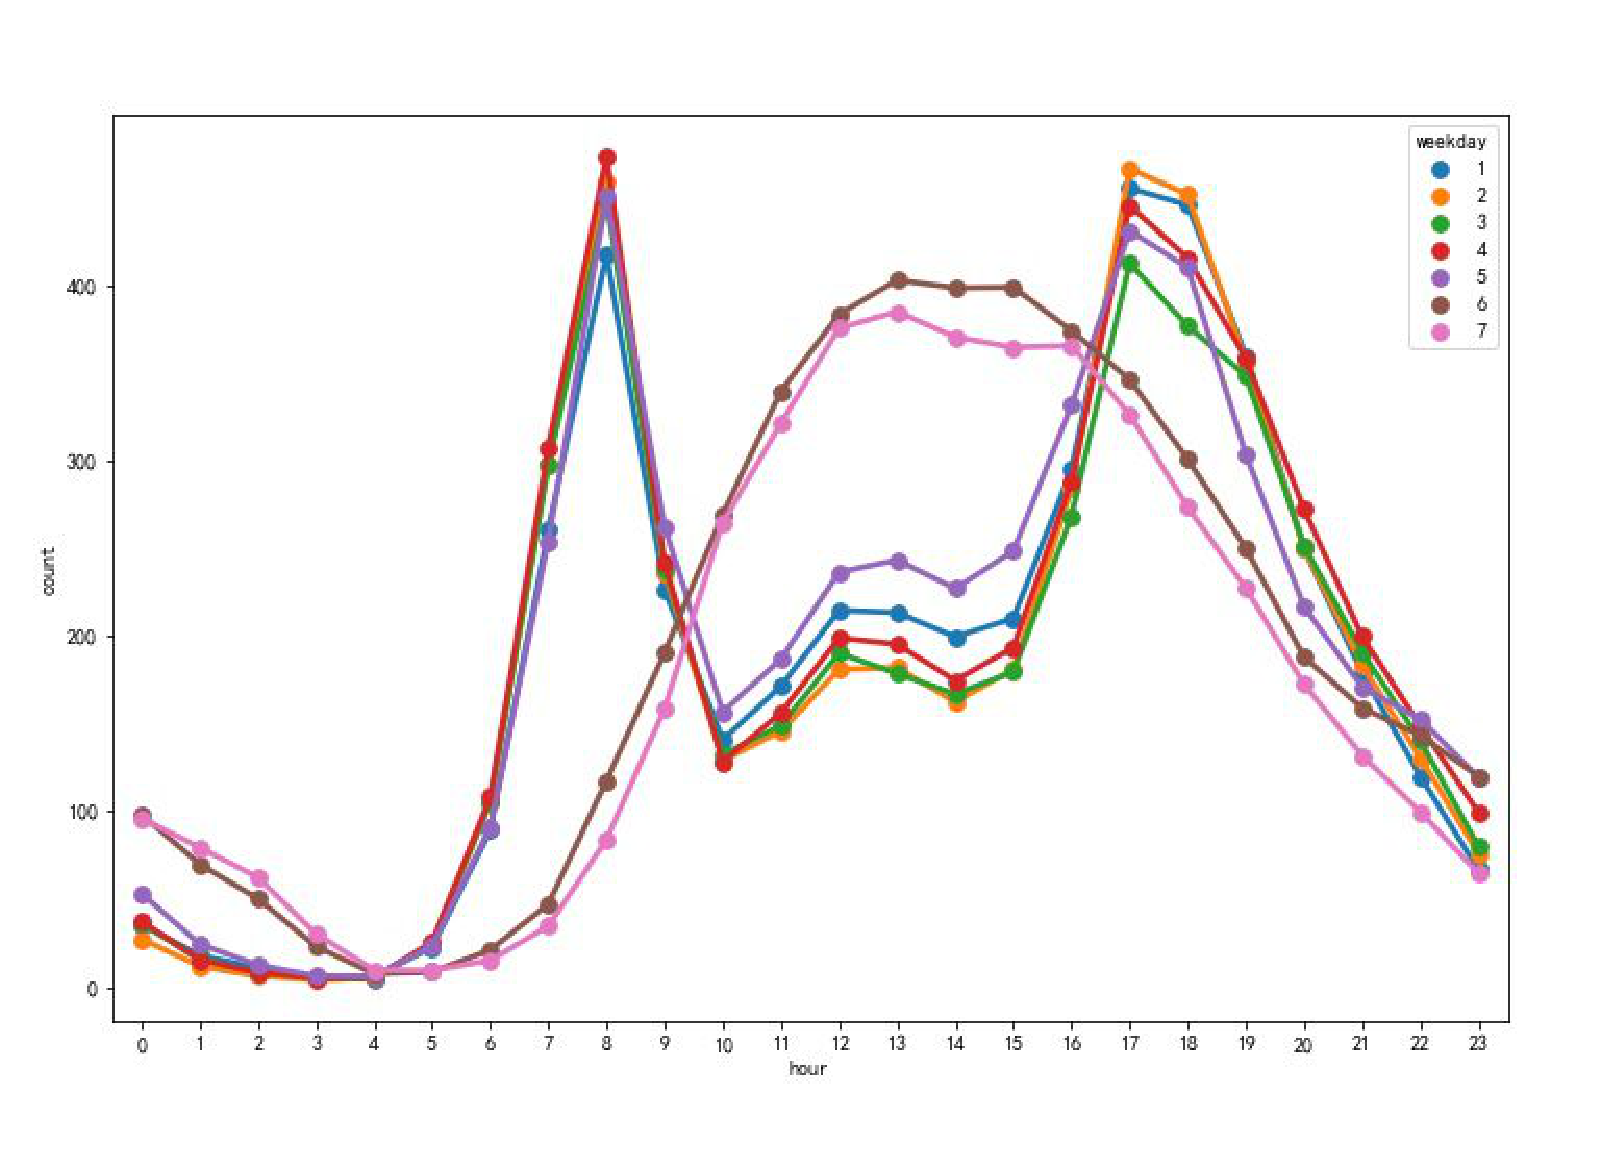
\includegraphics[width=0.7\textwidth]{pic/three hour2 (1).eps}
  \end{minipage}
  \hfill
\end{center}
 
(8)  Draw the thermal diagram of the correlation coefficient

\begin{center}
  \begin{minipage}{1\linewidth}
    \centering
    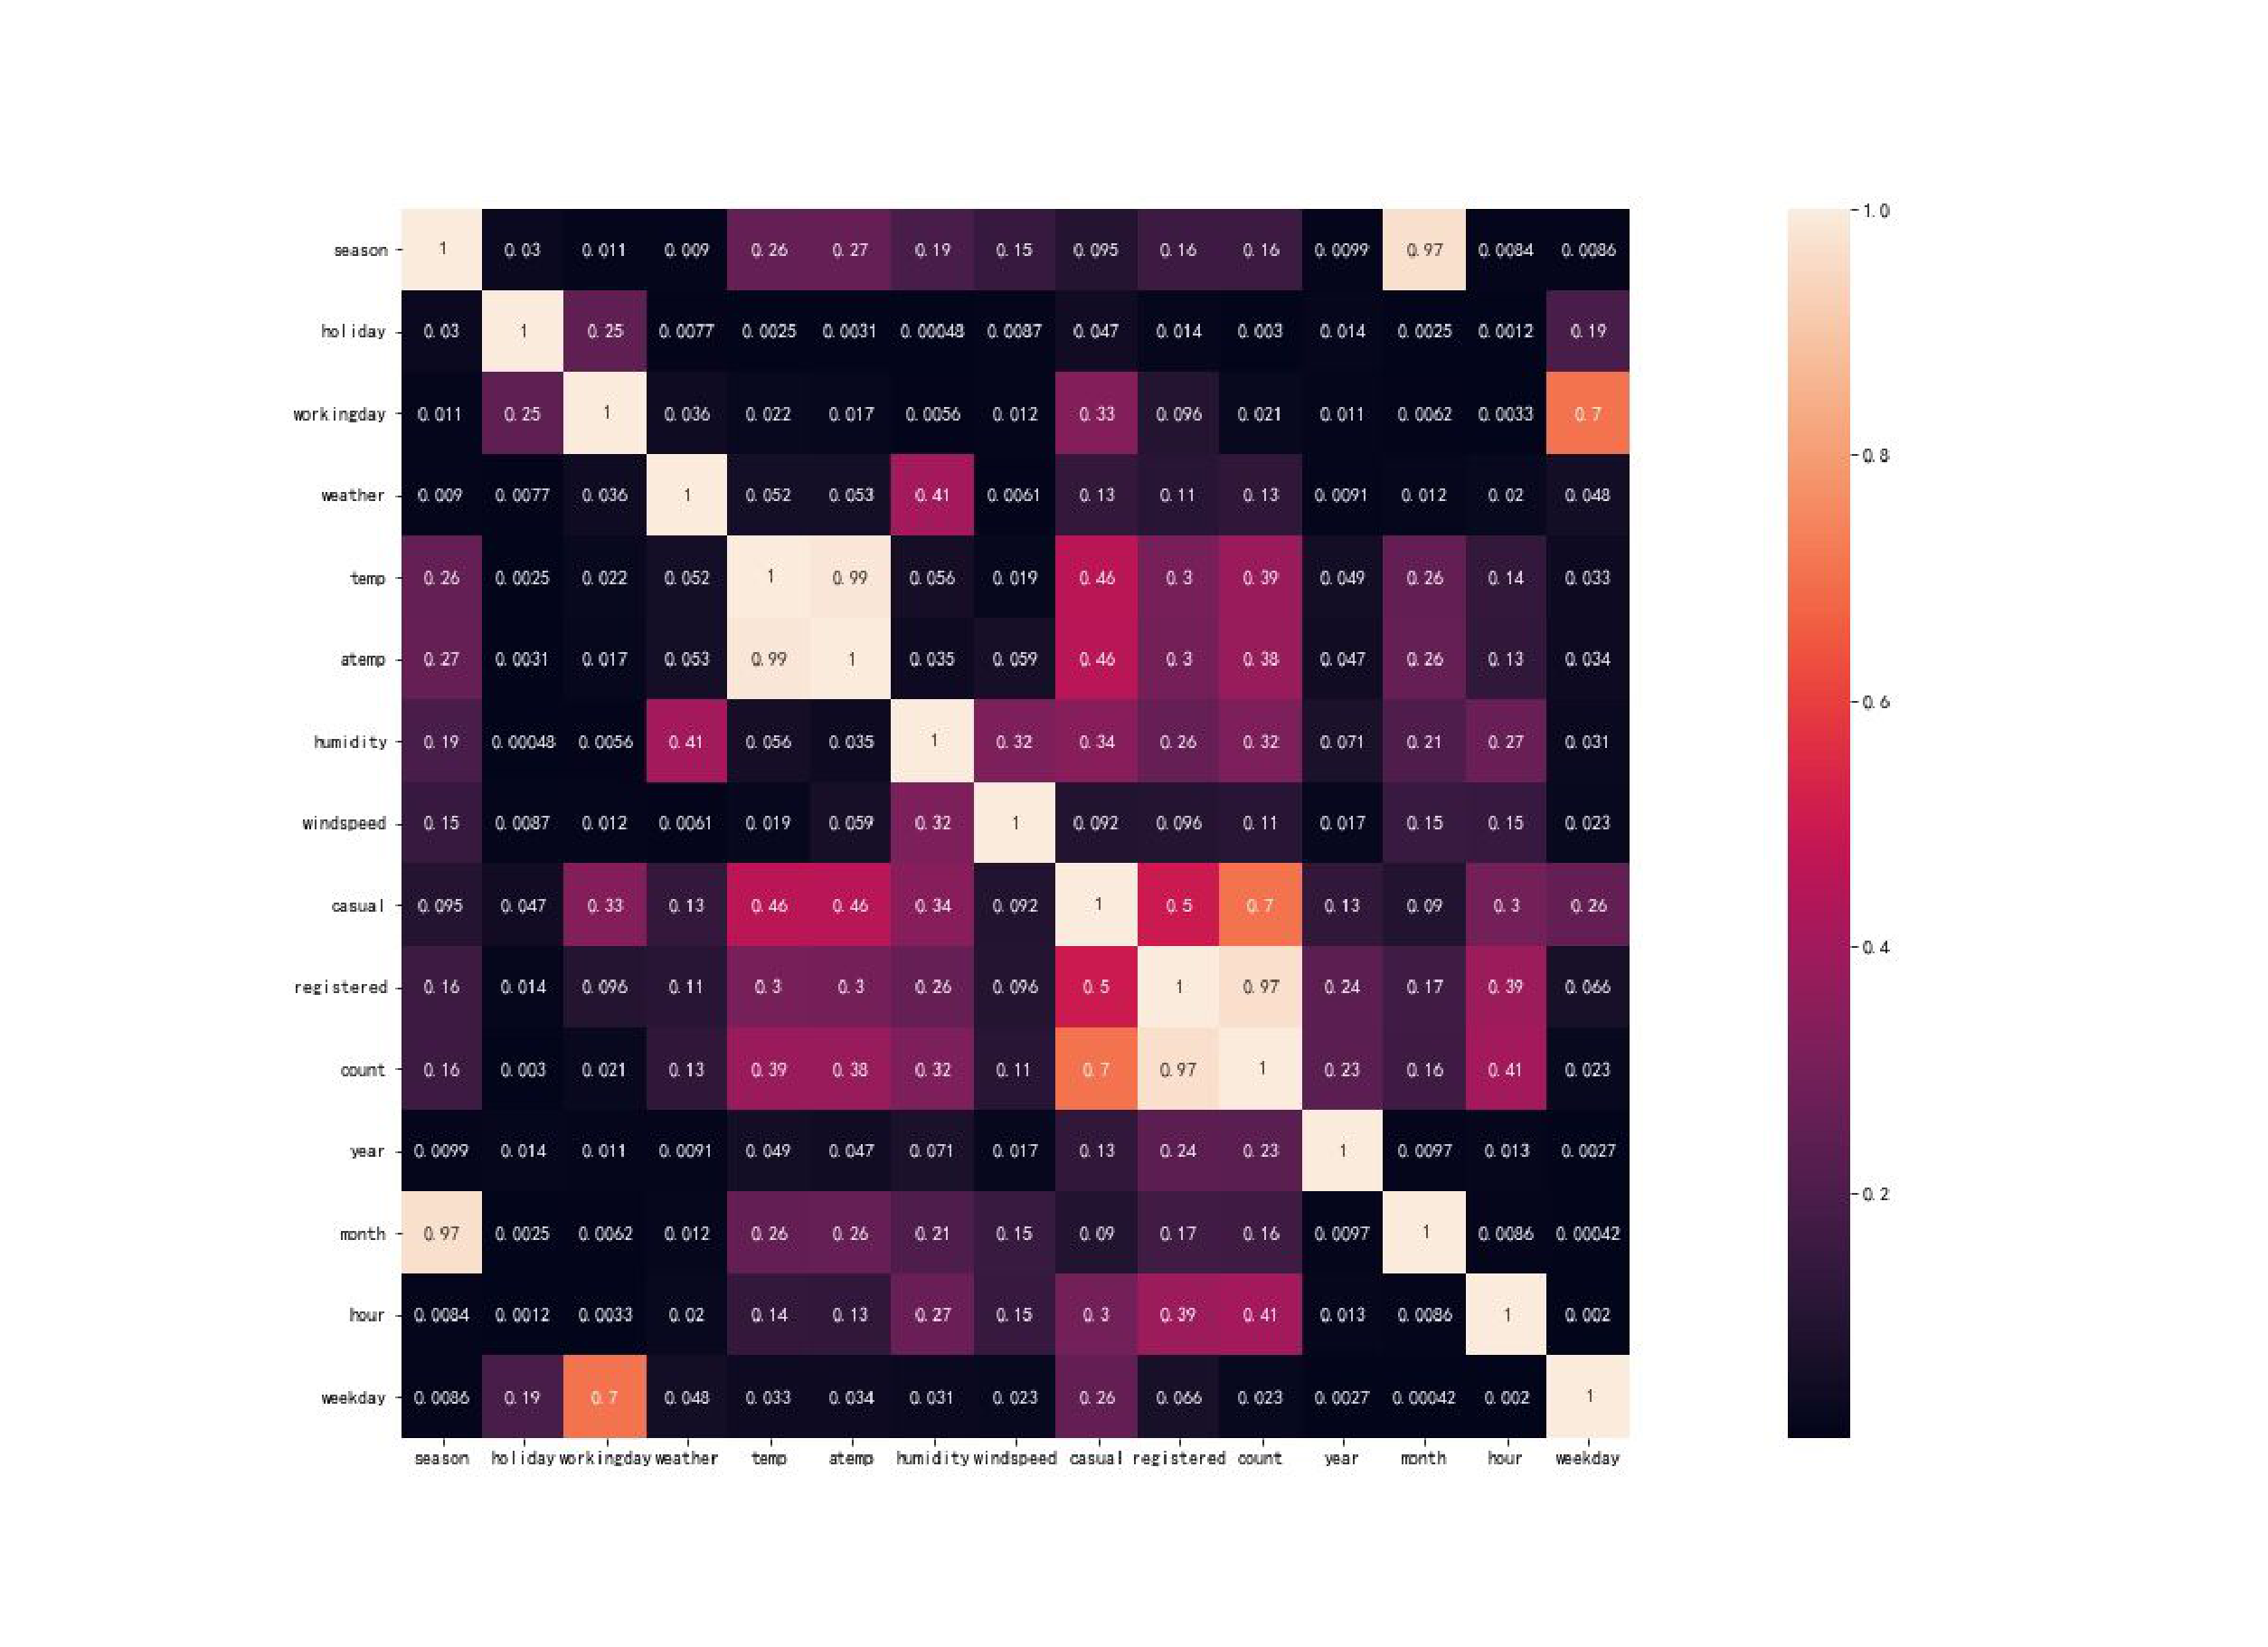
\includegraphics[height=0.5\textwidth]{pic/hot (1).eps}
  \end{minipage}
  \hfill
\end{center}


\begin{center}

  \begin{minipage}{0.3\linewidth}
  \centering

 % \includegraphics[width=0.9\textwidth]{logos/1 (3).eps}
  
  {\small{cost}}

  \end{minipage}
\end{center}


\section{Build Model}
1.Separate the training set and test set.\\
2Remove unwanted eigenvalues:'casual','count','datetime','registered','date','atemp','month','year','season','weather'\\
3.Cross validation is used to determine the optimal parameters.\\
4.View the selected optimal parameters:{'max_depth': 20, 'n_estimators': 150}\\
5.Apply the optimal parameters to the model, it can be obtained\\
Accuracy on test set:  0.6945996275605214\\
Recall rate on test set: 0.7379725915789399

\section{Conclusions}

Through this Kaggle project, I practiced by myself to have a deeper understanding of data visualization and to explore the structure and rules of data by means of drawing and tabulating.


% ----------------------------------------------------------------
\newpage
\bibliography{tuliplab,yourbib}
% TODO: you should change this yourbib into a proper bib file name

\bibliographystyle{plainnat}
%=================================================================

\listoftodos
Jupyter Notebook,Visual Studio Code,Latex,Git.
\end{document}

